\section{Constant Density Flow}
For the velocity profile shown as below\footnote{Here I used the
transformation of reference frame to make $U_0=(U_1-U_2)/2$ in
\eqref{kh:pro} without the loss of generality.}
\begin{equation}\label{kh:bg}
\mathbf{U}(z) =
\begin{cases} U_0 \mathbf{i} &\text{if $z>0$,}\\
-U_0 \mathbf{i} &\text{if $z<0$.}
\end{cases}
\end{equation}
with $\rho=\rho_0$ everywhere and the boundary conditions $\phi \to
0$ as $z \to \pm\infty$, the solution of the Reyleigh's Stability
equation \eqref{kh:ray2} is in the form
\begin{equation*}
\phi =
\begin{cases}
Ae^{-\alpha z} &\text{if $z>0$,}\\
Be^{\alpha z} &\text{if $z<0$.}
\end{cases}
\end{equation*}
There are two more boundary conditions at $z=0$:
\begin{enumerate}
  \item[(i)] The pressure at the interface must be continuous. From \eqref{kh:3-1}
  \begin{equation}
  \frac{\hat{p}}{\rho_0}=\frac{dU}{dz}\phi-(U-c)\frac{d\phi}{dz}\quad\text{is continuous.}\label{kh:b1}
  \end{equation}
  \item[(ii)] The displacement of the perturbed interface must be continuous. Let $z=z_0+\xi(x,t)$ be
  the displacement of the interface. The movement of the interface is given
  by
  \begin{align*}
  w'&=\frac{D\xi}{Dt}=\frac{\partial\xi}{\partial
  t}+(\mathbf{u}\cdot\nabla)\xi,\qquad
  \text{where }\mathbf{u}=\mathbf{U}(z)+\mathbf{u}'
  \end{align*}
  Apply the linearization to drop the product of perturbed terms,
  let $\xi(x,t)=\hat{\xi}e^{i\alpha(x-ct)}$
  \begin{align}
  w'&=\frac{\partial\xi}{\partial t}+U\frac{\partial\xi}{\partial
  x}=-i\alpha c\,\xi+i\alpha U\xi\notag\\
  \hat{w}&=i\alpha(U-c)\hat{\xi}\notag\\
  -\hat{\phi}&=(U-c)\hat{\xi}\notag\\
  \frac{\phi}{U-c}&=-\hat{\xi}\quad\text{is continuous at $z=0$.}\label{kh:b2}
  \end{align}
\end{enumerate}
Apply the boundary conditions from \eqref{kh:b1} and \eqref{kh:b2},
I get
\begin{subequations}\label{kh:lin}
\begin{align}
    (U_0-c)(-\alpha)A&=(-U_0-c)(\alpha)B\label{kh:lin1}\\
    \frac{A}{U_0-c}&=\frac{B}{-U_0-c}\label{kh:lin2}
\end{align}
\end{subequations}
Solving \eqref{kh:lin}, The solution is
\begin{equation}\label{lh:c}
    \boxed{c=\pm i U_0}
\end{equation}

The result is plotted in Figure \ref{kh1}. There is one unstable
mode and one decaying mode corresponding to positive and negative
value of $c_I$ respectively. In Kelvin-Helmholtz instability, every
wave number $\alpha$ has a corresponding unstable mode.
\begin{figure}[htpb]
  \centering
  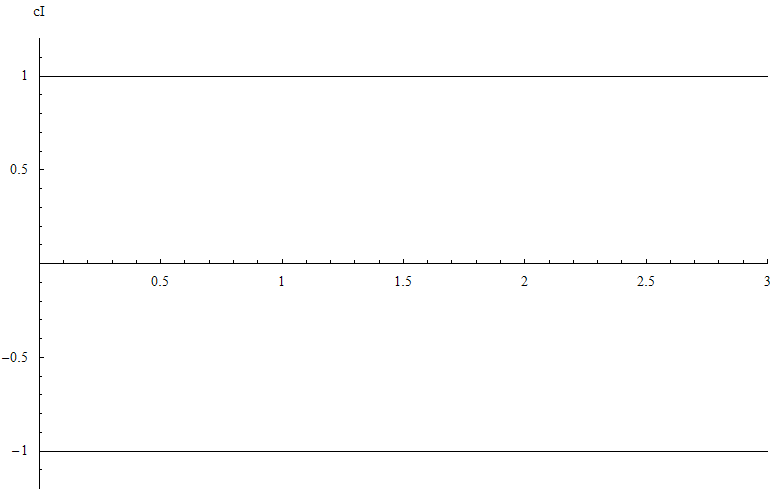
\includegraphics[width=0.5\textwidth]{kh1.png}\\
  \caption{$c_I$ vs.~$\alpha$ for $U_0=1$ of a KH mode}\label{kh1}
\end{figure}
